\documentclass[12pt]{article}
\usepackage[a4paper,margin=2.5cm]{geometry}
\usepackage{graphicx}
\usepackage{setspace}
\usepackage{tikz}
\usepackage[spanish]{babel}
\usepackage[T1]{fontenc}
\usepackage{lmodern}
\usepackage{amsmath}
\usepackage{hyperref}

\begin{document}
\thispagestyle{empty}

% ---------- CARÁTULA ----------
\thispagestyle{empty}
\begin{center}
    \vspace*{\fill}

    {\Large \textbf{Universidad de San Andrés}}\\[0.8cm]

    {\Huge \textbf{Inferencia y Estimación}}\\[0.6cm]
    {\LARGE \textbf{Trabajo Práctico N.º 1}}\\[1.5cm]

    \begin{tikzpicture}
      \node[draw, rounded corners=6pt, inner sep=14pt, line width=0.8pt]
      {
        \begin{minipage}{0.78\textwidth}
          \begin{center}
            {\Large \textbf{Compresión de Imágenes}}\\[0.8cm]
            {\large \textbf{Profesores:} Matías Perlin, Pau García Gulisano, Juan Ponce}\\[0.4cm]
          \end{center}
        \end{minipage}
      };
    \end{tikzpicture}

    \vspace{1.6cm}

    {\large \textbf{Integrantes:}}\\[0.4cm]
    {\large Máximo Barral -- Legajo 36585}\\[0.2cm]
    {\large Lautaro Valentín Caminoa -- Legajo 36571}\\[0.2cm]
    {\large Franco Sandri -- Legajo 36530}\\[1.4cm]

    \vspace*{\fill}
\end{center}
\newpage

% ---------- NUMERACIÓN DE PÁGINA ----------
\setcounter{page}{1}    % comienza numeración en 1
\pagestyle{plain}       % Número centrado

% ---------- INTRODUCCIÓN ----------
\section{Introducción}
En épocas de \textit{big data}, el volumen de información generada y almacenada crece a un ritmo exponencial. Dentro de este escenario, la compresión de información (y en particular de imágenes) se convierte en un proceso esencial para optimizar el almacenamiento, reducir costos de transmisión y mejorar la eficiencia en el procesamiento de grandes volúmenes de información visual. El \textit{análisis de componentes principales} (PCA, por sus siglas en inglés) constituye una de las técnicas más utilizadas para la reducción de dimensionalidad. Su fundamento radica en identificar las direcciones de mayor varianza en los datos y proyectar la información en un subespacio de menor dimensión, preservando la mayor cantidad posible de la variabilidad original. 

El objetivo del presente trabajo es implementar PCA en el contexto de compresión de imágenes, evaluar su desempeño mediante métricas cuantitativas y estudiar la relación entre la correlación espacial de los píxeles y la eficiencia de la compresión. Con ello, se busca profundizar tanto en la comprensión teórica del algoritmo como en su aplicación práctica en el análisis moderno de datos visuales.

% ---------- METODOLOGÍA ----------
\section{Metodología}
El trabajo se abordó en cuatro etapas, alineadas con la consigna:

\subsection*{(1) Correlación entre píxeles vecinos}
Para dos imágenes de prueba se construyeron vectores \((X_1, X_2)\) con pares verticales de píxeles (bloques \(2\times 1\)). La función \texttt{extraer\_pares\_verticales} toma filas de a dos sin superposición (\texttt{range(0, height-1, 2)}), y para cada columna forma el par \((\text{píxel superior}, \text{píxel inferior})\). Se hicieron gráficos de dispersión y se estimó el coeficiente de correlación con \texttt{np.corrcoef}. Para analizar la descorrelación de las variables en \(\mathbb{R}^2\), se aplicó una proyección PCA exploratoria (solo en este ejercicio).

\subsection*{(2) Compresión por bloques con PCA}
Se tomó una tercera imagen y se:
\begin{enumerate}
  \item Recortó al centro para que sus dimensiones fueran múltiplos de \(8\) (\texttt{cut\_img}).
  \item Segmentó en bloques \(8\times 8\) y se aplanaron por columnas (\texttt{order="F"}) en vectores de dimensión \(m=64\) (\texttt{n\_segmentation\_img}).
  \item Implementó PCA \textbf{desde cero} mediante SVD propio:
  \begin{itemize}
    \item Centrado \(X \leftarrow X-\mu\).
    \item Covarianza \(C=(X^\top X)/(n-1)\).
    \item Autodescomposición de \(C\): \(\,C V = V \Lambda\), autovalores \(\Lambda\) en orden decreciente.
    \item Valores singulares \(S=\sqrt{\Lambda\,(n-1)}\), y \(U = X V S^{-1}\) en las componentes no nulas.
  \end{itemize}
  \item Se eligió el número de componentes a retener \(k\) a partir del \emph{Space Saving} \(S\) (porcentaje de memoria ahorrada). En el código:
  \[
    k \;=\; \mathrm{round}\big(m\,(1-\texttt{saving})\big).
  \]
  Para \(m=64\) y \(\texttt{saving}=0.8\), se obtiene \(k=13\).
  \item Se proyectó \(X\) en el subespacio \(k\)-dimensional: \(Y = X V_k\).
\end{enumerate}
Se graficaron los autovalores en escala logarítmica, destacando los \(k\) conservados frente a los descartados.

\subsection*{(3) Descompresión}
Se revirtió la proyección con \( \widehat{X} = Y V_k^\top + \mu \). Luego, se rearmó la imagen colocando los bloques reconstruidos \((8\times 8)\) en su posición original (usando \texttt{reshape(..., order="F")} para reconstruir cada bloque siguiendo un orden de lectura por columnas). Se compararon visualmente imagen original y reconstruida.

\subsection*{(4) Medidas de desempeño}
Para una cuarta imagen se evaluó el MSE para \(S=\{5n: n=1,\dots,19\}\). Se graficó MSE vs. \(S\) y se mostraron reconstrucciones para \(S=\{75,80,85,90,95\}\).

Las métricas usadas:
\[
\mathrm{MSE}=\frac{1}{N_w N_h}\sum_{i=1}^{N_w}\sum_{j=1}^{N_h}\big(p_{ij}-\widehat{p}_{ij}\big)^2,
\qquad
S=\Big(1-\frac{k}{m}\Big)\times 100\%.
\]

% ---------- RESULTADOS ----------
\section{Resultados}
\subsection{Ejercicio 1: Correlación entre píxeles vecinos}
Los coeficientes de correlación estimados fueron:
\[
\rho_{\text{Imagen 1}} = 0.9792,
\qquad
\rho_{\text{Imagen 2}} = 0.1459.
\]
La Imagen 1 presenta fuerte correlación entre píxeles contiguos (alta redundancia), mientras que la Imagen 2 muestra correlación baja (mayor variabilidad). Tras una proyección PCA en \(\mathbb{R}^2\), los pares quedaron desacoplados (nube más “circular” y alineada a ejes), evidenciando la eliminación de redundancia lineal.

\begin{figure}[h!]
    \centering
    \includegraphics[width=\textwidth]{Ejercicio1a.png}
    \caption{Imagen y dispersión de pares verticales para ambas imágenes.}
    \label{fig:ej1a}
\end{figure}

\begin{figure}[h!]
    \centering
    \includegraphics[width=\textwidth]{Ejercicio1b.png}
    \caption{Dispersión tras la proyección PCA en \(\mathbb{R}^2\) (desacople).}
    \label{fig:ej1b}
\end{figure}

\subsection{Ejercicio 2: Compresión mediante PCA}
Con \(m=64\) y \(\texttt{saving}=0.8\), el algoritmo retuvo \(k=13\) componentes principales. El espectro de autovalores decrece con rapidez, indicando que pocas componentes concentran la mayor parte de la varianza. En la Figura~\ref{fig:ej2} se diferencian en azul los autovalores retenidos y en rojo los descartados.

\begin{figure}[h!]
    \centering
    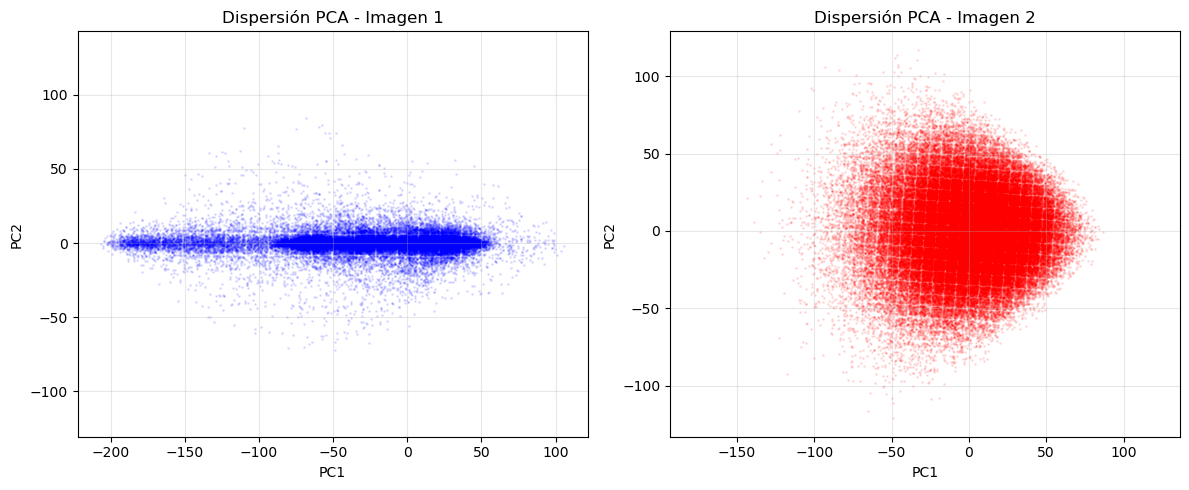
\includegraphics[width=0.8\textwidth]{Ejercicio2.png}
    \caption{Autovalores de la covarianza por bloques (\(8\times 8\)); conservados vs. descartados.}
    \label{fig:ej2}
\end{figure}

\subsection{Ejercicio 3: Descompresión}
La reconstrucción a partir de \(Y\), \(V_k\) y \(\mu\) produjo una imagen muy similar a la original, con algunas pérdidas en detalles finos y texturas, típicas de truncar componentes de menor varianza.

\begin{figure}[h!]
    \centering
    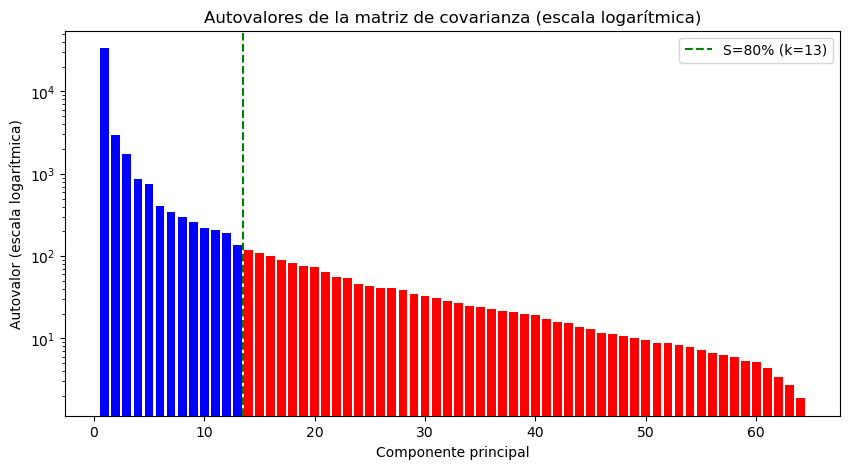
\includegraphics[width=\textwidth]{Ejercicio3.png}
    \caption{Comparación visual: original (izq.) vs. reconstruida (der.).}
    \label{fig:ej3}
\end{figure}

\subsection{Ejercicio 4: Medidas de desempeño}
El MSE creció de forma constante con el ahorro \(S\): al retener menos componentes (mayor \(S\)), aumenta el error de reconstrucción. La relación exacta depende del contenido de la imagen; ver curva MSE vs. \(S\) en la Figura~\ref{fig:mse}. Las reconstrucciones de la Figura~\ref{fig:ej4b} ilustran la degradación progresiva al pasar de \(S=75\%\) a \(S=95\%\).

\begin{figure}[h!]
    \centering
    \includegraphics[width=\textwidth]{Ejercicio4a.png}
    \caption{MSE en función del ahorro de espacio \(S\) (\(5\%\) a \(95\%\)).}
    \label{fig:mse}
\end{figure}

\begin{figure}[h!]
    \centering
    \includegraphics[width=\textwidth]{Ejercicio4b.png}
    \caption{Reconstrucciones para \(S=\{75,80,85,90,95\}\).}
    \label{fig:ej4b}
\end{figure}

% ---------- DISCUSIÓN ----------
\section{Discusión}
En el Ejercicio 1 se observó que la correlación entre píxeles vecinos influye directamente en la compresibilidad de una imagen: a mayor correlación, mayor redundancia y, por lo tanto, más posibilidades de reducir la información sin perder calidad.

El análisis de autovalores en los bloques de \(8 \times 8\) mostró que gran parte de la variabilidad de la imagen se concentra en unas pocas componentes principales. Esto justifica el uso de PCA para reducir la dimensión de los datos.

La implementación propia del algoritmo mediante SVD permitió cumplir con la consigna y controlar de manera explícita la cantidad de componentes retenidas. Los resultados indicaron que, al aumentar el porcentaje de compresión \(S\) (y por lo tanto disminuir \(k\)), el error de reconstrucción medido por el MSE crece y la calidad visual se deteriora, principalmente en los detalles más finos.

En conjunto, los experimentos mostraron que PCA es una buena herramienta para compresión de imágenes, logrando un balance razonable entre ahorro de espacio y calidad de la reconstrucción.


% ---------- CONCLUSIONES ----------
\section{Conclusiones}
El trabajo permitió comprobar que la correlación entre píxeles vecinos tiene un rol central en la compresión de imágenes: cuanto mayor es esta correlación, más eficiente resulta el uso de PCA para reducir datos sin comprometer la calidad visual. 

Los experimentos mostraron que gran parte de la información de la imagen puede conservarse reteniendo solo unas pocas componentes principales. En particular, con un ahorro del 80\% (conservando 13 de 64 componentes) se logró un buen equilibrio entre espacio utilizado y fidelidad de la reconstrucción. 

Finalmente, el análisis del MSE evidenció cómo la calidad se degrada progresivamente al aumentar el porcentaje de compresión, confirmando la relación esperada entre el número de componentes retenidas y el error en la reconstrucción.

\end{document}